\noindent
Now that we have a clear idea of both the domain and numerical representation of words, we may define an adversarial derivation of textual data in the context of a classification model, $f$.  As per the definition of an adversarial derivation, we need only to define the model difference, $\epsilon$, as well as the domain metric, $d_D$ and codomain metric, $d_C$.  We will consider primarily two definitions.\\

\noindent
The discrete metric is given by

\[
\rho(v,v^*) =
\begin{cases}
0 & \text{if $v = v^*$} \\
1 & \text{if $v \neq v^*$} \\
\end{cases}
\]

\noindent
\textbf{Definition.} Let $\{v_i\}_{i=1}^N$ be the sequence of vectors obtained from a given word embedding and text sample, then a discrete adversrial derivation is defined has having domain metric, $d_D(v,v^*) = \sum_i^N\rho(v_i,v_i^*)$, codomain metric $d_C(f(v),f(v^*)) = \rho(f(v),f(v^*))$, and difference $\epsilon = 1$

That is, a discrete adversarial derivation, $\{v_i^*\}$, of sample $\{v_i\}$ is the sample which changes the least amount of words possible, while changing the classification.  This definition is simple, though it may not yield very good results if solved.  For example, a positive movie review, ``This movie was good'' could easily be changed to a negative review by changing just one word resulting in ``This movie was bad''.  These two samples would obviously have different sentiments if read by a human.

Clearly the codomain metric, $d_C$ and difference, $\epsilon$ make sense for any defintion in this context, but the domain metric has room for improvement.  One possibility is to instead use Euclidean or Manhattan distance between word vectors, that is, $ d_D(v_i,v_i^*) = ||v_i-v_i^*||_2$ or $d_D(v_i,v_i^*) = ||v_i-v_i^*||_1$.  If we minimize this objective, then we would tend to use semantically similar words in substitution.  However, this does not necessarily solve the problem of actual sentiment inversion.  For instance, in our embedding the semantically closest (measured with the $l^2$ norm) word to ``bad'' is ``good.''  This makes sense since they are semantically very similar and would be used in the same contexts, but may result in obvious semantic flips.  We therefore look to other metrics in an attempt to find better results.  We found that for our sentiment classification model, the Jacobian was related to the sentiment of the word, which motivates the following definitions.\\

\noindent
\textbf{Definition.} Let the gradient of a model output, $f_i$, with respect to an input vector, $v$ be denoted by $g=\nabla_v(f)$.  The total gradient is given by 
$$g_t = \sum_{i=1}^D \nabla_v(f)_i$$
The gradient norm is given by 
$$g_n = \sqrt{\sum_{i=1}^D |\nabla_v(f)_i|^2} = ||\nabla_v(f)||_2$$

Both of these measures, along with the gradient itself, are shown for a small excerpt for one of the text samples in figure \ref{fig:saliency}.  We see that the three words with the largest total gradients are ``loved'', ``good'', and ``bad'' which are all sentimental.  We provide motivation for these choices of measure with a very simplified probabilitic analysis.

Suppose that each of the embedding dimensions is distributed independently and identically across words, with some mean, $\mu$ and variance, $\sigma^2$.  Let $g = \nabla_u(f)$ for a given word, $u$ in the sample, then 

$$\E{g^Tv} = \E{\sum{g_iv_i}} = \sum{g_i\E{v_i}} = \mu\sum{g_i} = \mu g_t$$

\noindent
If we are interested in purposefully altering classification, however, we might be more interested in the expected maximum value of $g^Tv$, that is,

$$Z(g) = \E{\underset{0\leq n\leq V}{\max}\,{g^Tv_n}}$$

\noindent
Unfortunately, there is no simple expression which captures this value.  However if we assume that $v_{n,i}$ is distributed normally, we have 

$$\E{\underset{0\leq n\leq V}{\max}\,{g^Tv_n}} = \E{\underset{0\leq n\leq V}{\max}\,{\sum_{i=1}^D{g_i}v_{n,i}}} = \E{\underset{0\leq n\leq V}{\max}\,{p_n}}$$

\noindent
Where $p_n \sim \mathcal{N}(\mu g_t,\sigma^2 g_n^2)$  There is still no closed form expression for this value, but there is a known upper bound:

$$Z(g) \leq \mu g_t + \sigma g_n\sqrt{2\log{V}}$$

\noindent
This inequality is intuitively satisfying.  It says that the maximum obtainable perturbation grows with both the vocabulary size and the norm of the gradient.  The total gradient also plays a role here, increasing or decreasing the expected maximum depending on the sign.

\begin{figure}
    \centering
    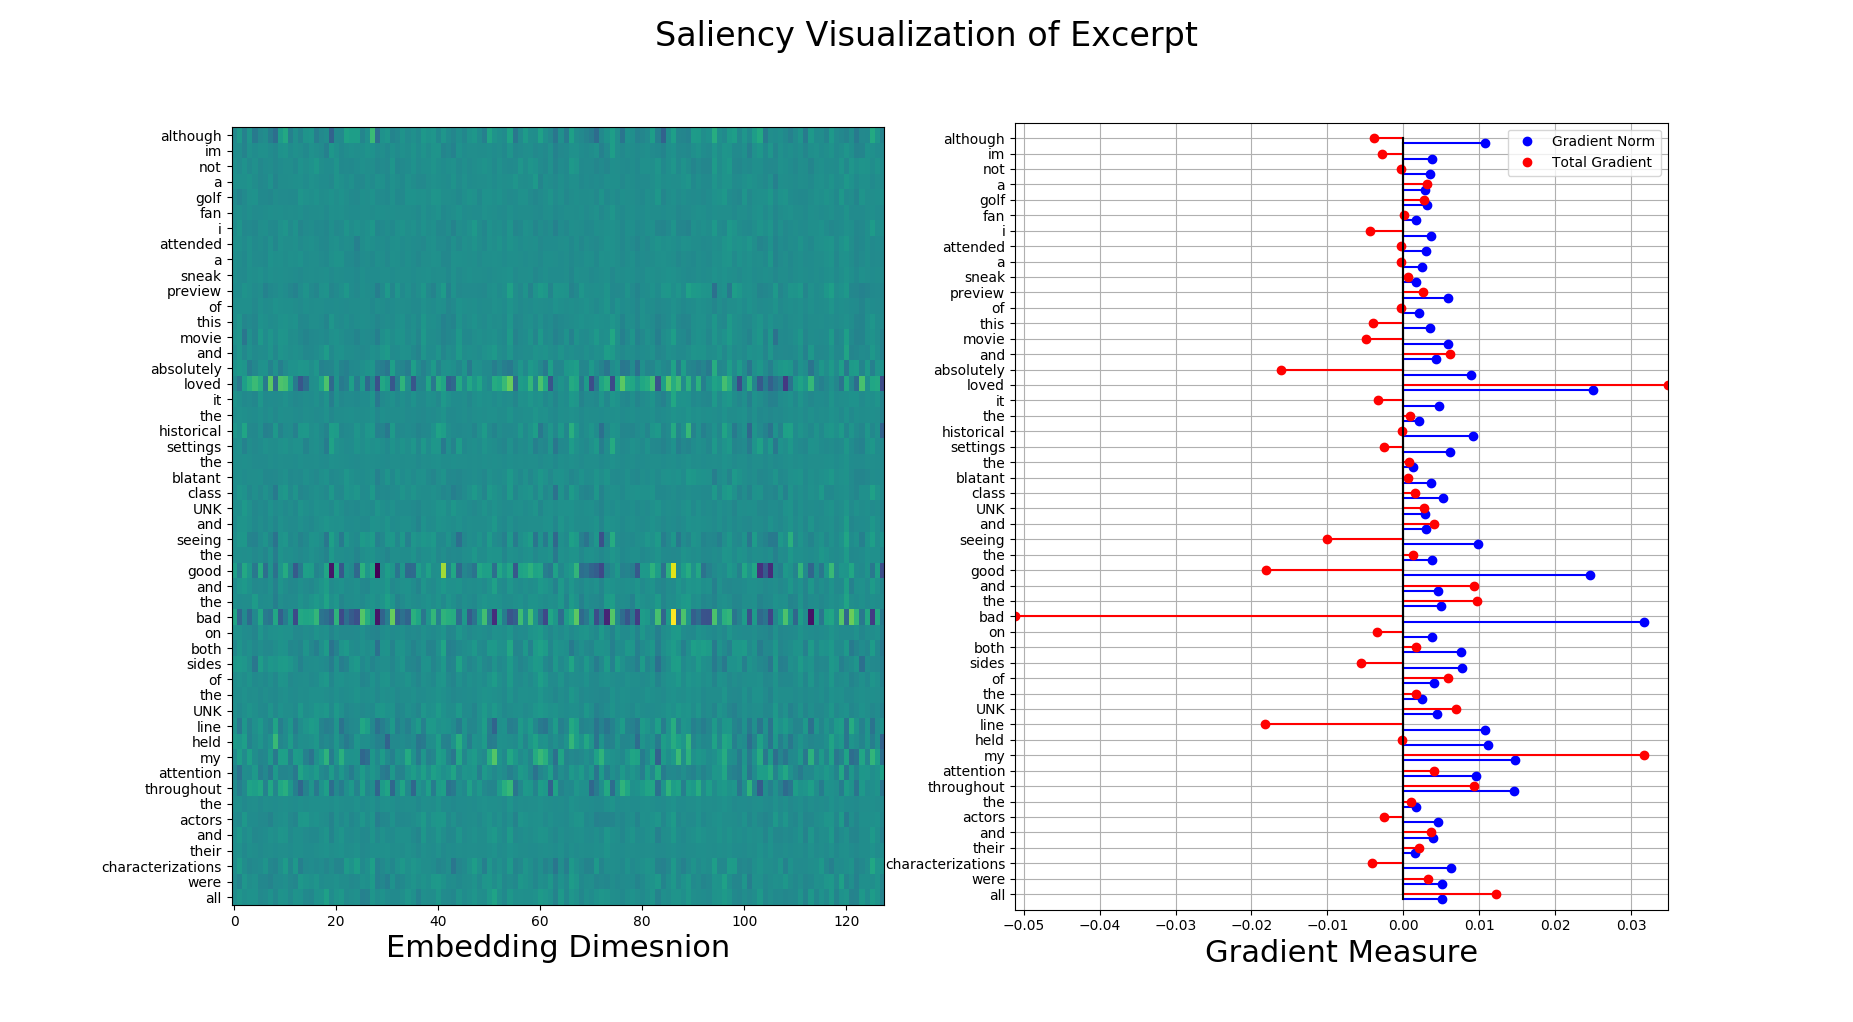
\includegraphics[width=\textwidth]{saliency.png}
    \caption{Different measures of word sentiment/importance}
    \label{fig:saliency}
\end{figure}
